\documentclass{ctexart}
\usepackage{bm, hyperref}
\usepackage{graphicx}

\begin{document}
\title{调研报告}
\author{马凯,金孜达,刘时,徐亦尧,李文睿}
\setcounter{tocdepth}{2}
\maketitle
\tableofcontents
\newpage

\section{项目成员}

马凯、金孜达、刘时、徐亦尧、李文睿。

\section{项目简介}

该项目提出一种可靠、实时、可伸缩、可扩展(可裁剪)、资源消耗低、面向流数据优化且能与网络集成的嵌入式文件系统,因此适用于多种物联网应用场景,尤其适用于资源有限的无线传感器网络的数据采集工作。

该文件系统的预期目标如下:
\begin{enumerate}
	\item 可靠性:在硬件故障情况下仍可正常工作,不会导致系统崩溃;
	\item 低资源消耗:适用于资源有限的设备;
	\item 可伸缩:插入新的闪存卡后将立刻为系统所用;
	\item 可扩展、可裁剪:根据自身需求,可配置是否需要某些功能;
	\item 面向流数据优化:适合存储和传输传感器抓取数据得到的流式数据;
	\item 网络集成:将数据写入相应文件即相当于将数据发送给服务器,毋须手动进行网络操作。并可在网络失去连接时自动在本地存储进行数据缓冲。
\end{enumerate}

通过提供一个接近标准文件 IO 的 API,实现物联网设备与中心节点的双向沟通。

本项目提出这样的问题:物联网需要怎样的文件系统?并将给出一个初步的答案。

\section{项目背景}

\subsection{物联网技术}

\subsubsection{物联网简介}

\begin{figure}
	\centering
	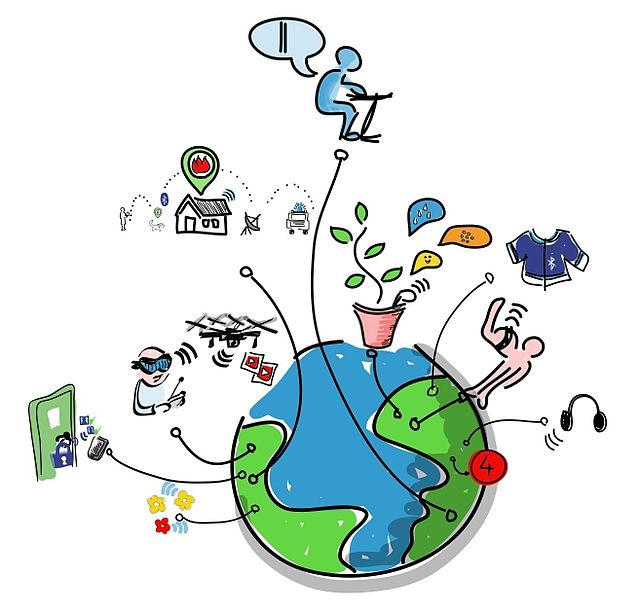
\includegraphics[scale=0.4]{Internet_of_Things.jpg}
	\caption{物联网示意图}
\end{figure}

物联网(Internet of Things)是物理设备、交通工具、家用电器及内嵌电子设备、软件、传感器、执行器和互联通性的设备的网络。每个东西都可唯一地通过其嵌入式计算系统识别,但也可以通过现有的互联网架构进行互操作。

传统互联网的信息来源严重依赖于人的输入,而人的精力有限,虽然物质世界的信息极为丰富,但人类无法尽数采取。因此物联网技术将物质与资讯连接,使得物品可以自主地采集信息并作出行动,依据信息进一步地反作用于物质世界。

在物联网上,每个人都可以应用电子标签将真实的物体上网联结,在物联网上都可以查出它们的具体位置。通过物联网可以用中心计算机对机器、设备、人员进行集中管理、控制,也可以对家庭设备、汽车进行遥控,以及搜寻位置、防止物品被盗等,类似自动化操控系统,同时透过收集这些小事的数据,最后可以聚集成大数据,包含重新设计道路以减少车祸、都市更新、灾害预测与犯罪防治、流行病控制等等社会的重大改变。

\subsubsection{物联网技术前景}

物联网将现实世界数位化,应用范围十分广泛。物联网拉近分散的资讯,统整物与物的数位资讯,物联网的应用领域主要包括以下方面:运输和物流领域、健康医疗领域范围、智慧环境(家庭、办公、工厂)领域、个人和社会领域等,具有十分广阔的市场和应用前景。

2016 年到 2017 年在线设备数量增长 31\% 达到 84 亿。专家预测,2020 年前,物联网将连接 300 亿个物体,预估全球市值将达 7.1 万亿美元。

\subsubsection{物联网技术简史}

早在 1982 年,就出现过智能设备网络的概念。卡内基梅隆大学的修改版可乐机成了第一个接入互联网的电器。

1991 年,Mark Weiser 中提出了“无处不在的计算”(Ubiquitous Computing)。1994 年,Reza Raji 进一步发展了这个概念,描述为“移动的小数据包发送到大的节点集,从而整合和自动化从家用电器到工厂的一切”。

1993 年到 1996 年之间,多家公司提出了自己的解决方案,如微软的 at Work 或 Novell 的 NEST。

然而,直到 1999 年该领域才得到了重视。术语“物联网”(Internet of Things)是由 Kevin Ashton 在 1999 年提出的。

\subsubsection{物联网设备及应用的特点}

\begin{figure}
	\centering
	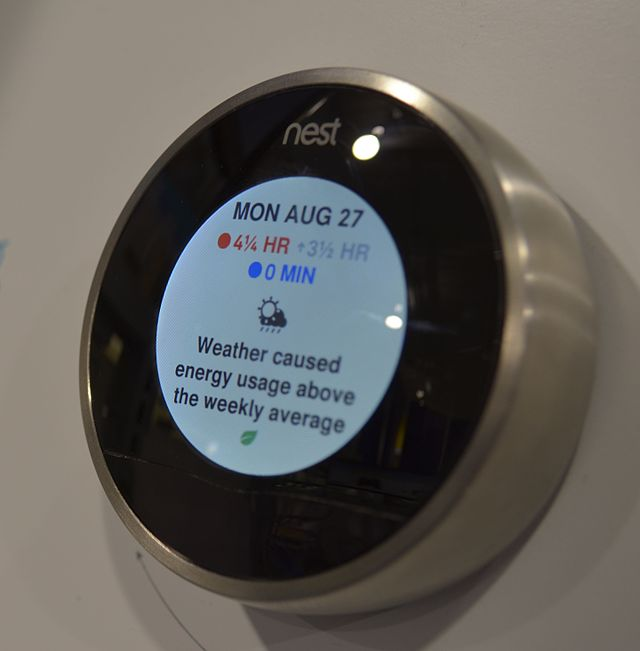
\includegraphics[scale=1.0]{Nest_Learning_Thermostat.jpg}
	\caption{Nest 学习型恒温器}
\end{figure}

\begin{figure}
	\centering
	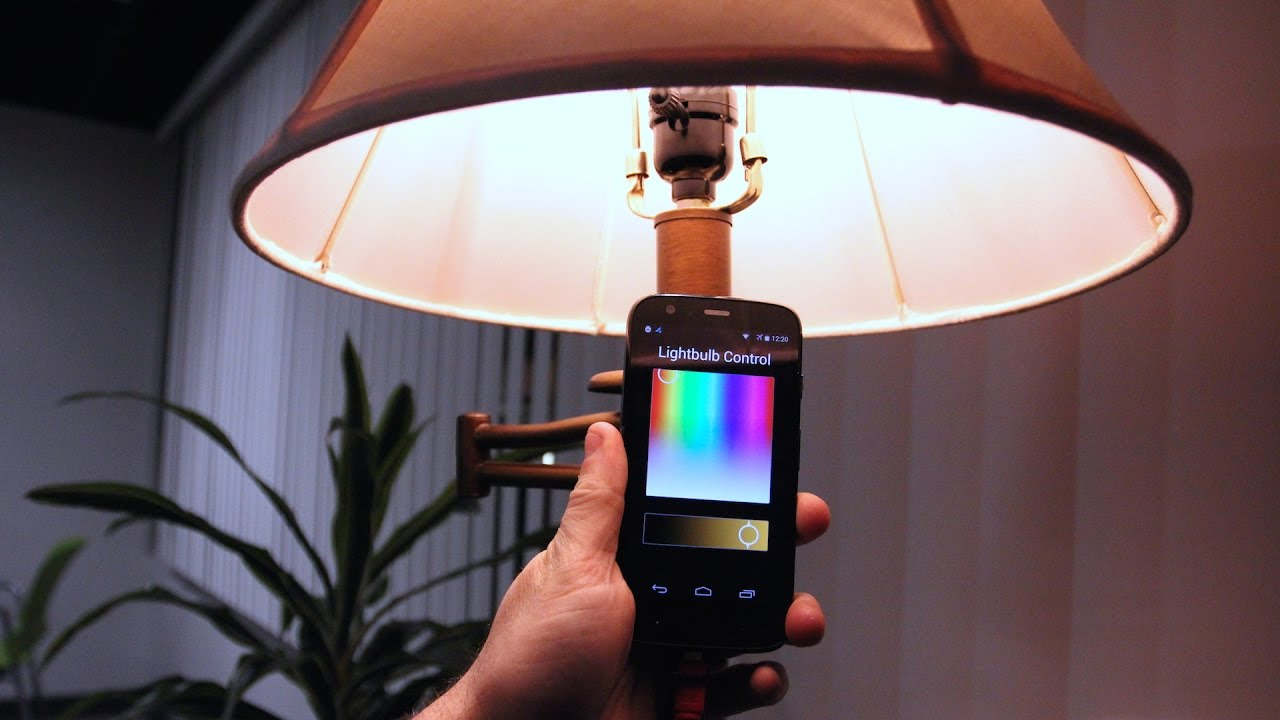
\includegraphics[scale=0.27]{Lightbulb.jpg}
	\caption{使用手机控制台灯的色彩和亮度}
\end{figure}

物联网设备的重要特点是硬件种类极为丰富,从低功率的 MCU 到新一代节能 32 位处理器都有。物联网应用的重要特点是需要可靠性、实时行为和与互联网的无缝集成。

这些需求对基础架构(如操作系统)开发者来说是重要的挑战。

\subsubsection{开发与推广应用中的困难}

目前,物联网是业界的热点,各种基础架构开发方兴未艾,生态尚不够成熟。从消费者层面来看,不同厂商的设备可能无法互相沟通,隐私和安全性也很值得担忧。

从开发者的角度来看,生态的不健全使得开发物联网应用难度不必要地高于开发相应的计算机软件。

\subsection{实时操作系统}

传统的操作系统以提高吞吐量(单位时间内处理数据的总量)为目标,从而在达到平均处理时间意义上的高性能。对响应时间有严格要求的软件系统在这种系统下无法合理地工作。例如,核反应堆监测系统需要有严格的响应时间限制,一旦某项任务超出了限制,将有可能导致整个系统崩溃,甚至对人的生命安全造成危害。由此可见,实时操作系统是以提高响应速度为目标,而不追求吞吐量,因此衡量一个实时操作系统坚固性的重要指标,是系统从接收一个任务,到完成该任务所需的时间,其时间的变化称为抖动。

可以依抖动将实时性分为三种:硬实时(Hard real-time)、严格实时(Firm real-time)、软实时(Soft real-time)。

\begin{itemize}
	\item[\textbf{硬实时}] 一旦出现某期限被错过的情况,即被视为系统失败。即所有任务必须在确定期限内完成。\\
	例子:美国的火星探路者因一个高优先级任务被低优先级任务阻塞,未在期限内完成,险些丢失。
	\item[\textbf{严格实时}] 允许不频繁的期限被错过的情况。即绝大部分任务在确定时间内完成。\\
	例子:装配生产线的机器人如果出错频率较低,造成的影响较小,可以认为任务是成功的。
	\item[\textbf{软实时}] 允许频繁的期限被错过的情况,只要错过期限。\\
	例子:传感器互相之间可以不同步,只要获取数据的时间足够相近,就可以认为是同时获取(而不是读取失败)。
\end{itemize}

物联网应用一般对实时性要求不高,达到软实时或严格实时一般即可满足要求。

\subsection{文件系统}

文件系统是用于控制数据存储和获取的操作系统的重要组成部分。与本项目有密切关联的两
种文件系统是嵌入式文件系统和分布式文件系统。

\subsubsection{嵌入式文件系统}

嵌入式系统强调资源消耗少、代码体积小,这在资源极为有限的嵌入式设备上是非常重要的。
此外嵌入式存储的一个重要特点是不使用磁盘,而多使用闪存盘,这决定了多数传统的用于
电脑的文件系统不适用于嵌入式系统。

嵌入式文件系统将闪存盘的地址空间转为命名空间,可以增强系统的可扩展性、和可维护性,
使项目可持续发展。

\subsubsection{分布式文件系统}

分布式文件系统与传统文件系统的区别在于,它不要求访问同一存储设备,而是使用网络协
议,允许通过组合多台普通机器达到单台强大机器的性能水准。

分布式文件系统的特点为:
\begin{enumerate}
\item 访问透明:客户端使用相同的接口对文件进行访问,并不知道文件是否在本机上;
\item 位置透明:提供一致的命名空间,不透露文件的位置信息;
\item 并发透明:如果一个进程修改了数据,其他客户端将看到修改;
\item 故障透明:服务器故障后客户端仍能正确工作;
\item 异构性:文件服务可被不同的硬件和操作系统平台提供;
\item 可伸缩:文件系统的规模可以小至一台机器,也可大至数千台机器;
\item 副本透明:文件可被透明地在服务器间被备份,而客户端毋须关心;
\item 迁移透明:文件可以被随意迁移,而客户端毋须关心。
\end{enumerate}

由此可见,一个全功能的分布式文件系统将对服务器和客户端的硬件提出较高要求,否则将
很难完成这些复杂的任务。

\section{立项依据}

\subsection{物联网设备为什么需要文件系统?}

一个物联网系统有多种拓扑形态。其中一种比较典型的形态是有一个性能强劲的服务器,用
于整合、分析、处理设备产生的数据,这种形态的应用也较为广泛:
\begin{itemize}
\item 传感器网络会产生大量数据,而这些传感器本身并不处理数据(或只是简单处理),
  随后将发给服务器进行同一分析、处理。
\item 在家庭智能化、办公室智能化等情景中,通常会有一个固定的服务器提供中心服务,
  其他设备与之连接,从而实现设备间的通信。
\end{itemize}

另有一种典型形态是物联网设备间互相组网。这种形态下设备本身性能应该是足够强的,所
以不作为本项目的重点。事实上,将本项目或传统的分布式文件系统推广到硬件资源强大的
设备间组网应该是比较容易的。下面我们的讨论也以第一种物联网系统形态,即服务器+大量
小型设备为落脚点展开:

首先,物联网设备系统中必然会产生文件,这些文件可能是系统本身的固件,可能是从远程
传输而来,也可能是为记录设备传感器采集的数据而生成。这就涉及到文件的存储与传输问题。

由于小型物联网设备的运算性能和存储空间都十分有限,目前有一种观点认为可以不在这类
设备上架构文件系统,而让存储直接在物理地址上进行,这样可以节省一定的设备资源。但
我们认为即便是小型物联网设备,仍然需要文件系统来实现文件管理:
\begin{itemize}
\item 扩展性:直接操作物理地址实现存储意味着设备的存储空间是固定不变的,但很
 多情况下我们希望存储是可变空间的。以传感器为例:在一开始设计时,我们希望在传感器
 上只要有很小的缓存空间即可,因为在理想的网络条件下,传感器产生的数据可以即时地发
 送到服务器。但在网络条件欠佳的环境下使用时,我们就希望可以给传感器外接一个存储设 
 备(u盘,micro tf卡等),来暂时缓存数据。文件系统使存储的扩展变成可能。
\item 兼容性:对于没有文件系统的设备,数据以二进制存储在物理地址空间中,这导致
 数据难以导出到现有文件系统:在向服务器传输数据时需要先将数据转换成可读的格式再发送;
 其存储设备在现有文件系统上也根本不可读。使用文件系统,可以免去数据传输时的转换步骤,
 也可以使直接通过存储设备获取物联网设备上的数据成为可能,便于用户获取和使用数据。
\item 组织性:数据在无文件系统的设备上的存储没有组织结构,导致数据不能有效地分级
 分类以便管理。如果在设备上架设了文件系统,这个问题就能得到很好的解决。
\end{itemize}

\subsection{现有文件系统的局限性}

为何不使用现有的文件系统?这是因为现有的文件系统都有一些不足之处,不适合物联网设
备使用\footnote{“不适合”是指不能满足物联网系统的一些需求,使得开发者需要手动开
  发一些支持程序库。}。

传统的用于计算机的文件系统有以下缺陷,使得这样的文件系统不能适用于物联网设备使用:
\begin{enumerate}
	\item 内存消耗过大:许多文件系统在内存中缓存大量数据,以加快文件操作;
	\item 不适合闪存:早期文件系统多面向传统的磁盘,数据常被放在一起,而适合嵌入式设备的闪存反而不适合这样的设计特点。由于成本原因,嵌入式设备的闪存一般不会搭载 FTL,这容易导致闪存磨损而寿命减少。
	\item 设计复杂:如层次式目录结构在用途比较单一的嵌入式系统中没有用处;日志等容易造成闪存磨损。最重要的是,过于复杂的实现会导致性能、能耗、资源消耗不能满足人意。
\end{enumerate}

物联网系统中嵌入式系统将直接接入网络,但若不搭载本地可擦写存储,普通的分布式文件系统也不能适用于物联网设备使用:
\begin{enumerate}
	\item 对网络要求高:物联网设备的网络环境一般并不稳定,一旦网络断开,在无本地存储的情况下数据将完全丢失。
	\item 对硬件性能要求高:分布式文件系统常常要求全功能操作系统,这在嵌入式设备上很难达到。
\end{enumerate}

此外,物联网设备还有传输流数据的需求,如传感器不断收集数据并不断发送到中心服务器。

\subsection{可能遇到的问题}
\subsubsection{硬件的差异性和应用的多样性}
嵌入式硬件与常见的个人电脑不同,其架构和性能的差别很大,其硬件谱从 8 位控制器到全功能的 64 位处理器均有覆盖,
RAM 资源可以从几十千字节到几百兆字节,这对我们项目来说是一个重要挑战。

\begin{figure}
	\centering
	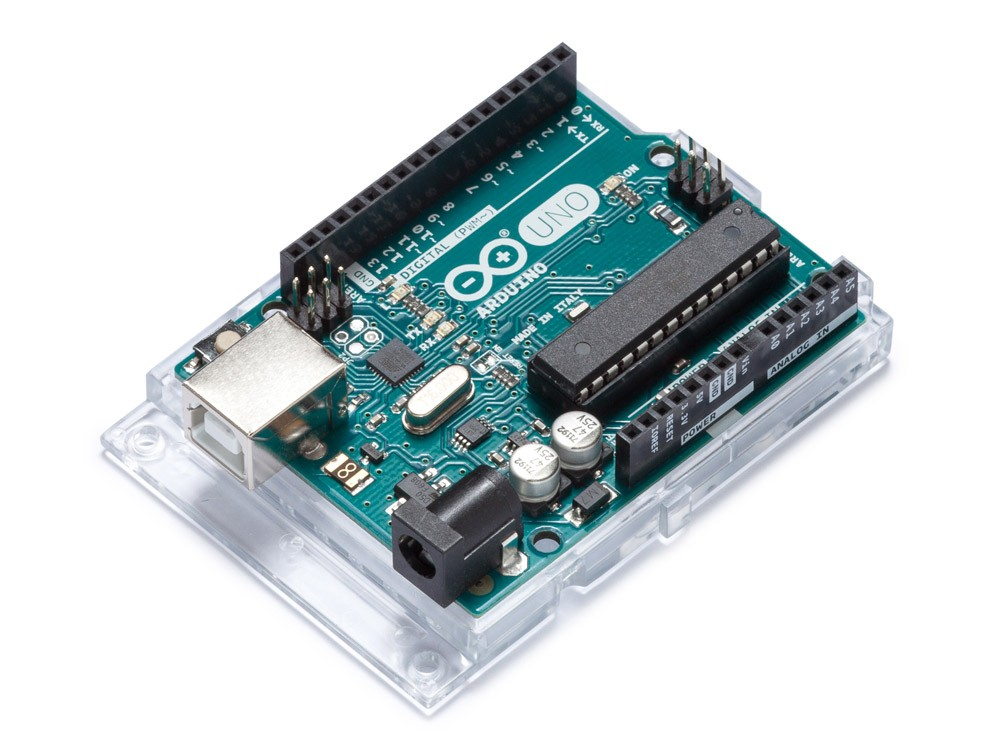
\includegraphics[scale=0.3]{arduino.jpg}
	\caption{Arduino Uno 采用 ATmega328 处理器,SRAM 仅 2KB,Flash Memory 仅 32 KB,EEPROM 仅 1 KB。}
\end{figure}

\begin{figure}
	\centering
	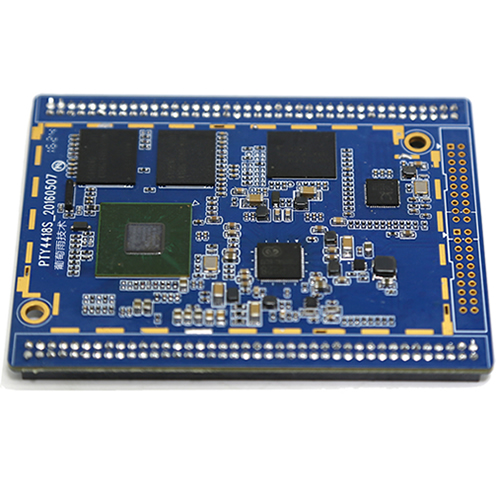
\includegraphics[scale=0.5]{ARM-Cortex.jpg}
	\caption{一款搭载 8 核 ARM Cortex A53 的硬件平台}
\end{figure}

嵌入式应用种类繁多,对文件存储、数据传输的要求也各有不同,如传感器需要快速可靠地传输流数据;而面向用户的应用程序则需要
存储多种不同格式的信息。

为此,本项目制定了可移植、可定制、自适应的目标,允许用户在不同的硬件平台上使用本项目成果,在满足硬件资源的要求下,给予
用户充分的自由选择自己所需的功能。从而可以在不改动源代码的情况下支持项目的无缝迁移和升级。但由于硬件和应用的差异十分大,
尽管我们进行了细致的考虑,仍会有部分场景无法覆盖,这将需要未来持续地关注和改进。

\subsubsection{嵌入式平台资源有限}
大多数嵌入式平台的资源都极为有限,这是因为嵌入式应用与硬件紧密配合:为了降低硬件成本,可以对应用代码进行修改;反过来,
若已有应用,则将选择能支持此应用的成本最低的硬件平台。

为此,本项目允许用户方便地裁剪出自己需要的子集,从而减小代码体积和内存占用。

\subsubsection{缓冲区的替换策略}
为支持不稳定网络下的透明数据传输,该项目预期提供自动缓冲功能,即在失去网络连接时将待发送数据在本地存储上进行缓冲,
从而可以在再次上线时重新尝试发送,减少重要数据的损失。但如果机器长期下线,由于本地存储极为有限,将出现缓冲区满的
情况,此时如何对数据进行取舍就成了重要的问题。

为此,本项目预期提供多种常见替换策略:
\begin{itemize}
 \item 丢弃:直接丢弃新数据,这种策略简单粗暴,但在部分情况下仍有实用价值,如在资源极为有限的情况下无法支持其他替换策略,而该策略已经可以减少数据损失;
 \item FIFO:丢弃最老的数据,这种策略适用于新数据优于老数据的场景,如温度计读取当前气温;
 \item 优先队列:丢弃优先级最低的数据(当所有数据优先级均一样时,使用其他替换策略),这种策略适用于数据优先级不定的场景,如传感器对数据采样,出现特定模式的数据优先级更高。
\end{itemize}
目前来看,这些策略都是可行的,具体实现有待进一步研究。

此外,用户提供替换策略也有价值:有时数据可以根据一定分布取样,从而选择保留最合适的数据,这种方案的可行性仍待论证。

\section{重要性和前瞻性}

本项目的提出围绕着这样一个问题:什么样的文件系统适合物联网?并将给出一个初步的答案。

本项目的核心任务是在满足嵌入式设备硬件限制下,实现一个能与物联网操作系统的网络栈
结合的文件系统。 从一种角度来看,它是增加了网络功能的嵌入式文件系统;从另一个角度
来看,它是适宜于嵌入式系统的分布式文件系统。

我们的预期目标是:首先,在资源受限的设备上建立起接近标准文件 IO 的 API,
实现物联网设备与中心节点的半透明\footnote{多数情况下毋须考虑网络问题,但客户端如
  果愿意,将可进行更细致的调整。}双向沟通(重点优化设备间流数据传输的性能),进而可以实现设备与设备间的间接沟通。这
样的设计将可满足很多典型物联网使用场景,如
\begin{enumerate}
\item 传感器的数据回传;
\item 家用智能电器的互相沟通;
\item 智能城市设备的互相沟通;
\item 等等。
\end{enumerate}
本项目的成果将可以大大降低开发此类系统的难度,提高此类系统的可扩展性和可维护性。

本项目将有望建立起一个标准化的信息存储和传输的流程,提供完整的开发平台,在充分利
用现有嵌入式系统和物联网的成果的基础上,搭建起一个让信息充分流动的平台,推动不同
物联网系统的互相整合,打破不同物联网之间的隔阂,建立起真正的“互联物联网”。

\section{相关工作}

为开展相关工作,我组在实时操作系统、嵌入式文件系统和分布式文件系统上进行了深入的调研。

\subsection{RIOT}

RIOT \footnote{http://www.riot-os.org/}是面向物联网的操作系统,致力于填补无线传感器网络的轻量级操作系统和传统的全面的操作系统之间的空白。其特性为:可靠、实时、自适应网络栈。

操作系统可以被三个关键特点描述:

\begin{enumerate}
	\item 内核的结构
	\begin{enumerate}
		\item 宏内核
		\item 分层方法
		\item 微内核
	\end{enumerate}
	\item 调度策略
	\begin{enumerate}
		\item 是否支持实时调度
	\end{enumerate}
	\item 编程模型
	\begin{enumerate}
		\item 所有任务执行在同一个上下文,内存地址空间没有分段
		\item 每个进程运行在自己的线程里,有自己的内存栈
	\end{enumerate}
\end{enumerate}

其中,编程模型也与开发者的开发体验紧密相关。

RIOT 实现一个继承自 FireKernel 的为内核架构,支持多线程及标准 API。此外,RIOT 也支持 C++ 和 TCP/IP 网络栈。RIOT 的优势为

\begin{enumerate}
	\item 高可靠性;
	\item 对开发者友好的 API;
	\item 模块化微内核架构使得单点故障无法影响整个系统。
\end{enumerate}

为了满足常数时间的要求,RIOT 内核大量使用静态内存分配(向用户程序提供动态内存分配接口)。调度器使用线程的循环链表,从而实现 $O(1)$ 的调度。常数时间的计时器操作利用了 MCU 通常会提供的多个比较寄存器。

为了减少 IoT 设备的耗电,RIOT 提供毋须任何周期性事件的调度器。当没有任务时,RIOT 执行 idle 任务,该任务将设备置于深度睡眠状态。

RIOT 中,上下文切换发生在两种情况
\begin{enumerate}
	\item 一个对应的内核操作被调用
	\item 一个产生线程切换的中断
\end{enumerate}
内核的低复杂度使得 RIOT 极为节能。

\subsection{LittleFS}

LittleFS 是适用于微控制器的小型故障安全文件系统\footnote{https://github.com/geky/littlefs},它用一种简单的方法实现了随机掉电时的文件一致性,使用写时复制技术,并且可以实现闪存磨损均衡。

\subsubsection{元数据}

LittleFS 将元数据储存在两个块上,每个块上有一个修订号,每修改一次则增加 1。使用简单的异或进行校验。进行修改时,首先选择最旧版本修改。一旦在此过程中掉电,要么版本号未增加,要么异或未修改,则可以检测到数据没有成功更新,而旧版本仍存在,可以成功读取。

\begin{figure}
\begin{verbatim}
  block 1   block 2        block 1   block 2        block 1   block 2
.---------.---------.    .---------.---------.    .---------.---------.
| rev: 1  | rev: 0  |    | rev: 1  | rev: 2  |    | rev: 3  | rev: 2  |
| data: 3 | data: 0 | -> | data: 3 | data: 9 | -> | data: 5 | data: 9 |
| xor: 2  | xor: 0  |    | xor: 2  | xor: 11 |    | xor: 6  | xor: 11 |
'---------'---------'    '---------'---------'    '---------'---------'
let data = 9             let data = 5
\end{verbatim}
\caption{LittleFS 元数据更新}
\end{figure}

\subsubsection{文件数据}

文件数据是一系列块的逆向链表,从尾部依次指向头部,从而实现 $O(1)$ 时间的追加。

当文件进行修改时,首先将被修改的块写到一个新块上,然后修改文件元数据,从而保证文件数据在掉电时的一致性。

\begin{figure}
\begin{verbatim}
  block 1   block 2        block 1   block 2        block 1   block 2
.---------.---------.    .---------.---------.    .---------.---------.
| rev: 1  | rev: 0  |    | rev: 1  | rev: 0  |    | rev: 1  | rev: 2  |
| file: 4 | file: 0 | -> | file: 4 | file: 0 | -> | file: 4 | file: 5 |
| xor: 5  | xor: 0  |    | xor: 5  | xor: 0  |    | xor: 5  | xor: 7  |
'---------'---------'    '---------'---------'    '---------'---------'
|                        |                                  |
v                        v                                  v
block 4                  block 4    block 5       block 4    block 5
.--------.               .--------. .--------.    .--------. .--------.
| old    |               | old    | | new    |    | old    | | new    |
| data   |               | data   | | data   |    | data   | | data   |
|        |               |        | |        |    |        | |        |
'--------'               '--------' '--------'    '--------' '--------'
update data in file        update metadata pair
\end{verbatim}
\caption{LittleFS 文件更新}
\end{figure}

由于逆向链表的顺序读取性能较差,LittleFS 让每个编号 $n$ 可以被 $2^x$ 整除的块逆向 $n-2^x$,从而实现最坏 $O(n \log n)$ 的读取。

\subsubsection{块分配}

传统的文件系统为分配空闲块需要维护一个空闲块列表,这会造成代码膨胀、内存占用多、BUG 多等问题。为此,LittleFS 不存储哪些块是空闲的,LittleFS 只需用所有的块减去正在使用的块即可。具体实现为:使用一个固定大小的前向检查位向量,每次分配时向前扫描,直到找到空闲块。

该方法的渐进复杂度为 $O(n^2)$,但实际使用时效率已经很好。如块大小为 4 KB 的 4 MB 的闪存芯片,只需 8 次扫描即可扫完整个闪存。

\subsubsection{目录}

目录使用树存储。由于内存极为有限,不能使用递归遍历内存,所以使用线索树存储。

\begin{figure}
\begin{verbatim}
            .--------.
            |root dir|
            | pair 0 |
            |        |
            '--------'
            .-'    '-------------------------.
           v                                  v
      .--------.        .--------.        .--------.
      | dir A  |------->| dir A  |        | dir B  |
      | pair 0 |        | pair 1 |        | pair 0 |
      |        |        |        |        |        |
      '--------'        '--------'        '--------'
      .-'    '-.            |             .-'    '-.
     v          v           v            v          v
.--------.  .--------.  .--------.  .--------.  .--------.
| file C |  | file D |  | file E |  | file F |  | file G |
|        |  |        |  |        |  |        |  |        |
|        |  |        |  |        |  |        |  |        |
'--------'  '--------'  '--------'  '--------'  '--------'
\end{verbatim}
\caption{LittleFS 目录数据结构示意图}
\end{figure}

\subsubsection{总结}

以上所述是 LittleFS 最基本的特征,它在一些细节上还有更仔细的考虑。LittleFS 是一个嵌入式文件系统的典型案例,它强调了设计的简单(从而达到体积小、效率高、BUG 少的目标),同时考虑了常见的使用场景,适合嵌入式系统使用。

\subsection{Google FS}
\subsubsection{GFS}
Google(gfs)是一个可扩展的分布式文件系统,用于大型分布数据密集型应用程序,在提供容错的同时运行在廉价的商品型硬件上,并为大量用户提供高集成性能。\cite{GFS}
\subsubsection{概况}
GFS是为Google日益增加的数据处理需求设计的,GFS与以前的分布式文件系统有着如性能,可扩展性,可靠性,可用性等很多共同的目标,但其设计由Google的应用工作负载和当前和预期的技术环境的关键观察所驱动,反映了一些早期的显着偏离文件系统设计假设,因此研究团队重新审视了传统选择并探索了根本上不同的观点。
\begin{itemize}
	\item 首先,组件故障是规范而非概念,由于数量庞大,某些组件会发生故障。持续监视,错误检测,容错和自动恢复必须要保证。
	\item 其次,系统上存储的文件大多都很大,定期处理大量TB级的文件时管理几十亿KB大小的文件是不切实际的,因此设计假设和参数要重新考虑。
	\item 第三,大多数文件都是以附加而不是覆盖的形式被修改,文件内的随机写入实际不存在,一旦被写入则只能被顺序读取,鉴于这种大型文件的访问模式,追加成为性能优化和原子性保证的重点,而在客户端缓存数据块则失去了吸引力。
	\item 第四,通过增加灵活性,共同设计应用程序和文件系统API可以使整个系统受益,如放宽了GFS的一致性模型,大大简化了文件系统,而不会给应用程序造成沉重的负担。还引入了一个原子追加操作,以便多个客户端可以并发地追加到一个文件中,而无需在它们之间进行额外的同步。
\end{itemize}
\subsubsection{设计综述}
\paragraph{设想}
\begin{itemize}
	\item 要定期监视检测故障,以及容错性和故障恢复
	\item 系统主要存储大文件,小文件也要支持,但不对其进行优化
	\item 两种文件读取方式:大型流阅读和小型的随机阅读
	\item 系统必须有有效的对同一文件进行并发附加的处理机制
	\item 高持续带宽比低时延更为重要
\end{itemize}
\subsubsection{Interface}
支持一般的创建、删除、打开、关闭、读写文件的功能。

GFS还支持快照和记录追加,记录追加可以让多个客户端同时向同一个文件追加数据而无需加锁。
\subsubsection{Architecture}
GFS由master和chunkservers组成,也可以轻易的在同一台机器上运行chunkserver和client。

文件被分为等大的块,每一块被64位的chunk handle(master根据块创建的时间产生)确定。每一块都在多个chunkserver上有备份,这样能确保稳定性,默认三份,用户可以指定备份级别。

master存储所有的元数据,如命名空间,访问控制信息,文件与chunk的对应关系,chunk的位置等,也控制系统级别的活动如垃圾清理,孤儿chunk的处理,chunk的合并等。master定期与chunkserver联系以传递指令和收集chunkserver的状态。

client则通过与master和chunkserver的沟通处理数据,将元数据处理交给master,而数据承载则直接交给chunkserver。

不论是client还是chunkserver都不缓存数据,因为这没有好处。
\subsubsection{single master}
用户添加文件时,直接将文件名及offset等信息发送给master,master添加文件信息并给client传回location及index,client再用此信息将文件传给chunkserver。
\subsubsection{chunk size}
chunk大小指定为64MB

好处:
\begin{itemize}
	\item 减少了client与master的沟通
	\item client可以在给定的chunk上进行更多操作,减少建立TCP连接需要的时间。
	\item 减少了master上元数据的大小。
\end{itemize}

缺点:hotspot
\subsubsection{metadata}
master上的metadata有namespace,文件与chunk的对应关系,chunk的位置。使用log使得系统升级更简单稳定。

master负责周期性的扫描,包括垃圾处理,错误恢复,为平衡负载的chunk合并等。

master不维护特定chunk的位置记录,只是在开始的时候与chunkserver通信,这解决了chunkserver的加入,离开,故障等时master与其的同步。

operation log包括元数据改变的历史记录,这非常重要,因此在远程的部分机器上也进行备份,master通过replay operation log来恢复文件系统状态。当log的size达到一定程度时,master检查状态,这样恢复的时候只要恢复最新的log上几条记录即可。checkpoint在能直接被map入内存的一个紧凑的B+树内,在启动时系统可以将log记录进新的log文件中,这样就不用delay启动期间的修改。checkpoint期间的fail不影响准确性,因为恢复操作会跳过未完成的checkpoint。
\subsubsection{Consistency Model}
GFS的一致性:
\begin{itemize}
	\item defined: 状态已定义,从客户端角度来看,客户端完全了解已写入集群的数据,例如,客户端串行写入且成功,此时的状态是defined
	\item consistent: 客户端来看chunk多副本的数据完全一致,但不一定defined,一般发生在多客户端并发更新时
	\item unconsistent: 多副本数据不一致
	\item undefined: 数据未定义
\end{itemize}
从修改过程看:
\begin{itemize}
	\item 串行over-write: over-write由客户端指定文件更新offset。当客户端是串行更新时,客户端自己知道写入文件范围以及写入数据内容,且本次写入在数据服务器的多副本上均执行成功。因此,本次写结果对于客户端来说就是明确的,且多副本上数据一致,故而结果是defined
	\item 并行Over-Write: 并行写入时多个客户端由于写入范围可能交叉而形成交织写。这时候,由于单个客户端无法决定写入顺序(只有主副本才能决定谁先写谁后写),因此,即使写入成功,客户端仍无法确定在并发写入时交叉部分最终写入结果,但是因为写入成功,所以多副本数据必然一致,即为consistent but undefined
	\item append: 客户端append操作无需指定offset,由chunk主副本根据当前文件大小决定写入offset,在写入成功后将该offset返回给客户端。因此,客户端能够根据offset确切知道写入结果,无论是串行写入还是并发写入,其行为是defined
	\item 在一系列的成功修改后,mutated file region被定义并且包含最后一次修改后的版本。之后按文件中的chunk顺序修改,并检测是否有过期的chunk,旧的chunk不会在与client通信时使用。
	\item 客户端缓存chunk的位置可能过期,于是client对缓存有时间限制,这会清除所有缓存信息。
	\item 组件的failure可能会损坏文件,因此GFS定期与chunkserver握手并使用checksum检查文件完整性,一旦出现问题,数据会迅速由其余可用的备份中恢复。除非在能够联系之前所有备份全部丢失,否则文件不可能彻底损坏(这种情况用户会收到error而不是损坏的文件)。
	\item 检查点允许编写者以增量方式重新启动,并无法成功处理在应用程序看来不完整的数据。
\end{itemize}
\subsubsection{租约(Lease)}
租约(Lease)是由GFS中心节点Master分配给chunk的某个副本的锁。持有租约的副本方可处理客户端的更新请求,客户端更新数据前会从Master获取该chunk持有租约的副本并向该副本发送更新请求。

租约本质上是一种有时间限制的锁:租约的持有者(chunk的某个副本)需要定期向Master申请续约。如果超过租约的期限,那么该租约会被强制收回并重新分配给其他副本。
\subsubsection{优点与不足}
\paragraph{优点}
负载均衡,容错性好,可扩展性强,满足POSIX语义,应用程序无需任何修改可直接使用GFS。
\paragraph{缺点}
Master启动时将所有元数据加载至内存中,由于gfs应用场景主要是大文件,对其影响并不严重,但限制了文件系统的可扩展性。

\subsection{星际文件系统}
\subsubsection{摘要}
星际文件系统(InterPlanetary File System,缩写IPFS,下用IPFS代替)是一个试图用相同的文件系统来连接所有计算机的端对端(P2P)分布文件系统。IPFS 与万维网的结构类似,但它也可以视作使用一个Git仓库交换数据的BitTorrent单群。 IPFS提供了一个高吞吐的区块存储模型,并带有基于内容寻址的超链接,从而形成一个广义的Merkle有向无环图。它由分布的散列表、带有激励机制的区块交换系统和自我认证的命名空间构成,没有单点故障,节点之间也不需要互相信任。
\subsubsection{IPFS 设计}
IPFS借鉴了以前端对端系统中的优秀想法,比如DHT,BitTorrent,Git和SFS等。在IPFS中,每份文件以及其中所有的区块都有一个唯一的指纹,被称作加密散列;IPFS对每个文件追踪历史版本并删除冗余的复制版本;每个网络节点无需存储全部数据,仅存储它感兴趣的一部分,以及一些索引信息来帮助它从其他机器上下拉数据;查询文件的时候,它通过网络来寻找含有此文件的节点;IPFS 使用星际命名空间(InterPlanetary NameSpace,缩写IPNS,下用IPNS代替)来将文件的散列映射为人类可读的名字。

IPFS 协议采用端对端模式,所有节点都是平等的。文件与数据结构统称IPFS对象。节点在本地存储IPFS对象并使用网络互相传递。 IPFS协议分为7个不同功能的子协议:
\begin{enumerate}
	\item 身份协议:管理节点身份生成与验证。
	\item 网络协议:使用各种已有的底层协议管理端对端连接。
	\item 路由协议:通过维护信息帮助定位特定的端或对象,同时对本地或者远程请求相应。
	\item 交换协议:使用新的区块交换协议(BitSwap)有效地分配区块,该协议类似于市场交易机制。
	\item 对象协议:使用Merkle有向无环图的结构,用链接来建立不可变动的对象,比如文件数据结构和交流系统等。
	\item 文件协议:一个类似Git的带版本管理的文件系统。
	\item 命名协议:一个自我认证的可变的命名空间。
\end{enumerate}
\paragraph{身份协议}
节点通过NodeID辨认身份,NodeID是通过S/Kademlia加密谜题来对公钥做散列得到的,公钥和私钥使用口令加密存储在各自的节点中。

在每次启动时,用户都可以选择实例化一个新的节点,不过这个操作会流失他们在网络上原先的累计收益,所以一般他们都愿意保留原先的节点。

在第一次连接时,双端交换公钥,并检查公钥的散列与NodeID是否一致,若不一致则拒绝连接。

IPFS 也接受使用多种散列函数,所以在交换公钥的时候也可以在头部加入自己的散列函数的代码。
\paragraph{网络协议}
通常,一个节点时常与数百个网络中的其他节点沟通信息,有时也可能会跨越整个网络。IPFS网络协议带有如下特性:
\begin{enumerate}
	\item 传输:IPFS可以使用任何传输协议,推荐使用WebRTC DataChannels或者uTP。
	\item 可靠性:如果下层的协议没有保证可靠性,那么IPFS也会提供可靠性。
	\item 连通性:使用ICE NAT遍历技术。
	\item 完整性:可选,使用散列校验和检查消息的完整性。
	\item 权威性:可选,使用发送者的公钥和HMAC算法确认消息的权威性。
\end{enumerate}
\paragraph{路由协议}
节点需要一套路由系统来帮助它们找到其他端的网络地址,以及那些可以提供特定对象的端。IPFS使用一个基于在S/Kademlia和Coral上的DSHT来达成此功能。IPFS DHT通过区块的大小区分它们的存储方法,例如小于等于1KB的区块DHT直接存储,大于1KB的区块DHT将存储引用信息(能提供此区块的对象的NodeID列表)。
\paragraph{交换协议}
IPFS使用BitSwap协议交换区块。类似于BitTorrent,BitSwap中的端有一条需求列表记录它想要的区块,也有一条提供列表记录它能提供区块。BitSwap的机制类似于一个永恒的市场,在这里节点可以自由地获取和提供任意存在的区块。一些区块可能来自于毫无关联的文件,不过节点也可以一起打包出售。

在BitTorrent里,为了防止有些节点只是抓取数据但从不提供,它使用了投桃报李的策略来惩罚这些节点。在BitSwap里也定义了类似的交换意愿。在端对端中,记债务比
\[
r = \frac{bits\_I\_sent}{bits\_I\_receive+1}
\]并定义发送意愿
\[ P_{(message\_willing\_to\_send|r)} = 1 - \frac{1}{1+e^{6-3r}}
\]
在每次发送或者接收数据后,更新r。可知,如果对方接受的数据与发送的数据的比例上升,那么我方的发送意愿将降低。当这个比例在1附近的时候,发送意愿大约在0.95;若比例提升到2,其意愿将降低到0.5;若比例超过3.6,则意愿迅速降为0.01以下。该策略可以防止通过大量创建全新节点然后纯粹为了拉取数据的行为。

BitSwap协议要求每个节点各自保存自己的一份账本存储这些信用信息,也包括自己的。在双端建立连接时,它们需要交换账本并保持信息一致。如果不一致,也可建立新账本,但会损失过去的信誉或债务。为防止恶意节点故意丢失账本来欺骗节点,对方也可以认为丢失账本者不可信,从而直接拒绝交易。

对象协议

DHT和BitSwap为IPFS构成一个庞大的端对端系统,用于快速可靠地储存和分布区块。IPFS建立了一个Merkle有向无环图,其将对象用加密散列连接起来。这是一个广义的Git数据结构。Merkle有向无环图为IPFS提供了许多有用的特性,如:
\begin{itemize}
	\item 内容寻址:所有内容都用它的多个散列校验和唯一定位。
	\item 防篡改:所有的内容都可通过校验和检验,IPFS可以据此检测被篡改或损坏的数据。
	\item 去重:拥有一致内容的对象视作等价,也只存储一次。
\end{itemize}
IPFS用散列唯一确定路径,所以以下路径都是等价的:
/ipfs/<hash of a>/b/c
/ipfs/<hash of b>/c
/ipfs/<hash of c>
\paragraph{文件协议}
IPFS的文件结构与Git非常接近,故不做表述。
\paragraph{命名协议}
IPFS使用内容来给文件寻址,但是文件是变动的,需要找到一种方法使得IPFS能在相同的路径找到变动的数据。IPFS认为,对象是永恒存在的,从而其采用了类似Git的版本管理,其中对象是不变的,但是引用确是可变的。

在IPNS中,为每个节点建立如下命名空间:

/ipns/<NodeID>

其下的内容不按照内容寻址方式建立,而是使用子目录路由协议。
\subsubsection{IPFS实际使用案例}
土耳其官方不能封禁的维基百科

土耳其在2017年4月封禁了维基百科。一些黑客行为主义者制作了一份维基百科的副本,并使用IPFS的方式在线发布。因为IPFS搜索内容的方式是从最近可用的副本中选择一个下载,用一个IPFS地址理论能找到任何一个副本,所以官方封掉一部分副本后,还可以找到另一份副本解决问题。

加泰罗尼亚独立公投网站复刻

加泰罗尼亚在2017年10月1日举行公投,此前几天,西班牙法院判定公投官网违法并予以阻拦。加泰罗尼亚海盗党使用IPFS复刻公民投票网并成功举行公投,随后在同年10月27日宣布独立。
\subsubsection{优点与不足}
\paragraph{优点}
分布式的文件系统减少了存储需求,版本管理使得历史可追溯,同时也可以设置成允许有多个副本,使得其能够做到更强的容错性,弱化垄断力量的介入,保证民主自由的进行。
\paragraph{不足}
路由的算法实质上在大网络里效率并不是特别高,而市场化的区块交易机制也依然会出现所有市场经济该出现的典型问题,且保存所有版本实质也增加了存储开销,在没必要保存历史的情况下是没有意义的。


\subsection{Gnutella 项目}
\subsubsection{关于 Gnutella 项目}
Gnutella是一个用于分布式搜索和数字资源共享的协议,他的特色是它的点对点、非中心的模型。

在这个模型中,任何一个客户端同时也是一个服务器,反之亦然。所以Gnutella中给它们起了一个专门的名字叫做servent (是从“SERVer”和“cliENT”各取一部分组成的)。Servent提供客户端接口,用户通过这个接口可以提交查询并查看查询结果,同时,它们也可以接受查询请求,在本地数据中检索,并返回符合条件的结果。因为这种分布式属性,实现Gnutella协议的由servent组成的网络具有高度的容错性,一部分servent掉线并不会中断正在进行的网络操作。
\subsubsection{Gnutella协议}
\begin{enumerate}
	\item 连接Gnutella网络(Bootstrapping过程)
	
	为了连接Gnutella网络,servent需要发现并存储多个主机的地址,有四种方式
	\begin{enumerate}
		\item 调用一个GWebCache。这是一个有人上传到他们的Web服务器的PHP脚本。运行在用户计算机上的Gnutella程序调用脚本来获取计算机的IP地址,并获取最近完成相同事情的程序的IP地址。这让Gnutella程序能够找到彼此。
		\item 在握手期间,Gnutella程序在X-Try和X-Try-Ultrapeers头文件中告诉对方更多的IP地址。
		\item 有些地址以相同的方式洒在Pong message(reply to ping(discover hosts on network))中。
		\item Query hit(reply to query)也包含IP地址。
	\end{enumerate}
	\item 启动算法
	
	一般情况下,在一个会话期内,不要向web cache发送太多的请求,查询GWebCache的次数不应该超过一次。也就是说,一个用户掉线的时候,代替的方案是用本地主机的cache来存储发现的主机地址,并和GWebCache一起使用。
	\begin{itemize}
		\item 启动客户端并调入本地主机cache
		\item 使用本地主机cache连接GNet.
		\item 如果在X秒后还没有连接到GNet,查询一个随机的GWebCache.
		\item 等待最少Y秒后,向另一个GWebCache发送请求。(在第一次选取的GWebCache死机或者反应非常慢的情况下)
		\item 在Y秒后,如果第一次GWC调用还没有返回结果,每隔Z秒调用一个新的GWC,直到收到其中一个的响应。
		\item 一旦至少收到一个GWC的返回结果,只有在本地主机cache为空的情况下,           servent才应该在接下来的session中发送新的请求 (如果软件提供初始的主机cache,并且没有清除主机cache的选项,这种情况就不应该发生).
	\end{itemize}
	假设X,Y和Z的值分别为5秒、10秒和2秒,这样应该能够确保servent能够很快连接到GNet并把查询GWebCache的次数控制到最低。
	
	启动过程还应该确保servent不用经常连接一个远程主机,每秒钟少于一次是一个合理的界限。为了达到这个要求,一个解决办法就是确保本地主机cache中总是有足够多的主机,这样就能保证任何一个主机都不会在一分钟之内被再次试图连接。
	
	每一个servent在握手时都应该发送一个X-Try头,这个头给出这个servent可以尝试连接的主机列表,允许它在不用调用GWebCache的情况下得到新的主机地址。例如:
	
	X-Try:  1.2.3.4:1234, 1.2.3.5:6346, 1.2.3.6:6347
	
	servent应该发送适当数量的主机,一般在10到20之间。这些随着X-Try头发送的主机信息应该是确切的。所以,servent应该只选择那些最近(在发送X-Try头之前几分钟内)所知还在运行的主机。如果最近发现还在运行的主机数量少于10个,那发送时就少发送一些。如果servent实现了响应cache(参见3.4节),在响应信息中发现的主机可以认为具有空闲的时隙。但这不适用于在监控QueryHits中得到的主机信息。这样,在返回信息中得到的主机信息可以替换X-Try头中主机的位置,而QueryHits中发现的主机却不行。
\end{enumerate}
\subsubsection{握手协议}
一个Gnutella servent通过与当前在网络上的另一个servent建立连接的方式把自己连接到Gnutella网络。一旦第一个连接建立起来,网络可以提供更多的当前连接在网上上的主机地址。在得到当前在网上的另一个servent的地址时,首先建立一个到servent的TCP/IP连接,然后开始一个握手的消息序列。客户端是发起连接的主机,服务器是接受连接的主机。

(以下步骤来自于网络)
\begin{enumerate}
	\item 客户端建立一个到服务器的TCP连接
	\item 客户端发送“GNUTELLA CONNECT/0.6<cr><lf>”
	\item 客户端发送带有所有域的头,除了供应商自定义的特殊域,每个域以\"<cr><lf>"结束,在整个头的最后添加一个额外的\"<cr><lf>"
	\item 服务器以"GNUTELLA/0.6 200 <string><cr><lf>"应答,这里<string>应该是"ok",但是servent应该只查找"200"这个代码作为状态标志。
	\item 服务器发送自己信息头的全部,按照3规定的格式
	\item 如果客户端在解析完服务器发送的信息头以后,还希望继续,就发送"GNUTELLA/0.6 200 OK <cr><lf>"给服务器作为应答,就像4一样。否则,它需要返回一个错误码,并关闭这个连接。
	\item 客户端发送供应商自定义的信息头,与3的格式一样。
	\item 客户端和服务器按照3和5中得到的信息,按照自己的要求发送和接收二进制消息。
	
	例如:
	First-Field: this is the value of the first field<cr><lf>
	Second-Field: this is the value<cr><lf>
	of the<cr><lf>
	second field<cr><lf>
	<cr><lf>
	
	下面是一个客户端和服务器交互的例子。从客户端发送到服务器的数据列在左边,从服务器发送到客户端的数据列在右边。
	
	\begin{tabular}{cc}
		\hline
		Client                          &Server\\\hline
		GNUTELLA CONNECT/0.6<cr><lf>& \\
		User-Agent: BearShare/1.0<cr><lf>& \\
		Pong-Caching: 0.1<cr><lf>& \\
		GGEP: 0.5<cr><lf>& \\
		<cr><lf>& \\
		&GNUTELLA/0.6 200 OK<cr><lf> \\
		&User-Agent: BearShare/1.0<cr><lf> \\
		&Pong-Caching: 0.1<cr><lf> \\
		&GGEP: 0.5<cr><lf> \\
		&Private-Data: 5ef89a<cr><lf> \\
		&<cr><lf> \\
		GNUTELLA/0.6 200 OK<cr><lf>& \\
		Private-Data: a04fce<cr><lf>& \\
		<cr><lf>& \\
		{[binary messages]}&{[binary messages]} \\ 
	\end{tabular}
\end{enumerate}

\subsection{百度文件系统(Baidu File System)}
\subsubsection{介绍}
百度文件系统(以下简称BFS)是一个为支持实时应用而设计的分布式文件系统。类似于其他分布式文件系统,BFS具有高容错性。但与此同时,BFS还兼具低读写延迟和高吞吐量的特性。\cite{BFS}
\subsubsection{特性}
\begin{enumerate}
	\item 持续可用性:Nameserver 多节点冗余,并使用Raft共识算法维护其一致性,单个节点宕机不影响整体可用性。
	\item 高吞吐:高性能的数据引擎能最大化IO的吞吐量。
	\item 低延时:全局负载均衡,自动检测并规避慢速节点。 //似乎尚未实现
	\item 可线性扩展:支持多数据中心的架设及1w+数据节点管理。
\end{enumerate}
\subsubsection{结构:共五层}
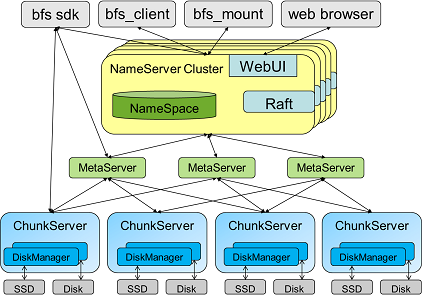
\includegraphics[width=\textwidth]{bfs.jpg}
由底至上:
\begin{enumerate}
	\item 硬件
	\item 单机节点ChunkServer:管理底层硬件
	\item MetaServer:为NameServer分担压力
	\item NameServer:类似于hdfs的namenode,但是一个集群而非单节点,这样可以解决部分可用性和性能瓶颈的问题。\footnote{hdfs中分Namenode和Datanode两种节点,是主从式结构。其中,Namenode负责管理文件系统的名字空间namespace以及客户端对文件的访问,而Datanode则负责节点存储。这种设计简化了系统的架构,因为存储数据无需经过Namenode。}
	\item 外层:用户接口/本地服务/sdk等
\end{enumerate}
\subsubsection{总体设计}
\begin{enumerate}
	\item 主备master结构:
	\begin{itemize}
		\item master之间通过一致性协议保持同步,每个master都存储所有信息。
		\item master的数据是落地(即被储存在持久化存储设备,如硬盘中)的,不一定非得全内存,通过LRU cache算法保证热点访问的快速响应。
	\end{itemize}
	\item 文件分块
	\begin{itemize}
		\item 文件是否分块决定了能否支持大文件
		\item 文件名信息是否存储在master决定了是否支持小文件
		\item 折衷是对大文件才分块,小文件(<100G)不分块;创建文件夹时指定可否list,可list的必须存在目录树中,不可list的可以哈希到chunkserver,让chunkserver去维护meta信息。
	\end{itemize}
	\item 文件meta信息(元数据:描述文件属性的数据)
	\begin{itemize}
		\item 文件meta信息存储在master会导致master负载过高(内存,cpu)。 我们选择对于不分块的文件,将文件meta存储在chunkserver,如果用户要list,那仅需要访问master,但如果要获取文件大小等信息,那就必须得访问对应的chunkserver了,master仅存储namespace和每个文件在哪些chunkserver上。
	\end{itemize}
	\item 写数据流
	有两个选择:
	\begin{itemize}
		\item client写一份,然后chunkserver通过复制链创建多副本,优势是client带宽占用低;
		\item client一次写多份,优势是可以多写一份,并在写的过程中抛弃慢节点。
	\end{itemize}
	\item 名称空间
	使用LevelDB存储:可以简单的将整个目录结构平展开,并提供高效的文件创建、删除、list和rename操作。例. 对于实际目录结构:
	
	/home/dirx/
	
	/filex
	
	diry/
	
	/filey
	
	/tmp/
	
	filez
	
	存储格式为:
	
	1home -> 2
	
	1tmp -> 3
	
	2dirx -> 4
	
	2diry -> 5
	
	3filez -> 6
	
	4filex -> 7
	
	5filey -> 8
\end{enumerate}
\subsubsection{Master(NameServer)高可用设计方案:}
\begin{enumerate}
	\item 背景:在BFS中,NameServer负责管理文件meta信息以及所有ChunkServer的状态信息,是整个系统中唯一拥有全局信息的模块,同时也成为了系统的单点。NameServer的不可用会直接导致文件系统的瘫痪,于是提高NameServer的可用性至关重要。
	\item 结构:将NameServer 扩展为集群,Client只与集群Leader进行交互。每一个NameServer中有一个同步模块(Sync),负责集群间的状态同步,保证元数据的一致性。
	\begin{itemize}
		\item Sync模块
		
		Sync模块主要有两个功能,选主和日志同步。选主操作就是在NameServer中确定唯一一个Leader,并且在Leader异常后迅速选出新任Leader。日志同步操作实际上就是同步NameServer中所有需要落地的数据写操作。Sync模块设计为与NameServer松耦合,仅暴露必须接口,内部可以采用任意一致性协议实现。这样的设计使得我们可以实现多种一致性方案,以满足不同程度的可用性及性能需求。当前我们采用Raft协议实现。
		\item Leader
		
		NameServer集群中的Leader负责接收和响应Client的请求,并把所做出的决定通过Sync通知集群中其他NameServer。Leader只在通知成功后才会向Client返回操作成功。
		\item Leader
		
		NameServer集群中的Leader负责接收和响应Client的请求,并把所做出的决定通过Sync通知集群中其他NameServer。Leader只在通知成功后才会向Client返回操作成功。
	\end{itemize}
	\item 主要流程操作方案:
	\begin{itemize}
		\item 对写操作(改变文件meta信息的操作,包括Create、Delete和Rename):
		
		同步结果的方案:Leader在收到操作后先对数据库打一个快照,检查完合法性后,在提交给Sync之前就将数据写入本地数据库。之后再将操作提交给Sync,Sync返回扩散成功后,Leader将快照删除并给向Client返回成功。在Sync返回成功前,所有的读请求都会读快照之前的数据,也就是说Client不会读到还未扩散成功的数据。
		
		同步操作的方案:Client向Leader Nameserver发起请求,Leader收到请求后,对所需操作的路径加锁,检查操作合法性。如果操作是合法的,Leader将需要落地的数据通过Sync扩散给从Nameserver。Sync模块返回扩散成功后,Leader向Client返回操作成功。从NameServer收到提交操作的指令后,无需检查操作合法性,直接根据指令执行操作更改状态机和内存结构。
		
		两种方案各自有一定的局限性:同步结果的问题在于当操作的结果很大(例如删除目录下所有文件),可能超出内存大小范围,从而很难保证操作原子性。同步操作基于一个假设:Leader和从NameServer将同一个指令应用到状态机及更改内存状态所产生的结果严格一致。
		
		对扩散的失败,例如RPC超时、写失败等需要重试处理,如果超过一定重试次数,则均视为Nameserver集群不可用,需人工介入处理。各一致性协议对于扩散失败的定义不同,例如Raft中,大于半数成员收到消息便认为扩散成功;主从模式中主或从任意一方写失败均认为是扩散失败。
		\item 对读操作:
		
		因为数据扩散存在延时,只有Leader掌握最新的数据,所以只有Leader可以响应Client的读请求。Client向Nameserver集群中任一实例发起读请求,如果正好是Leader接收到了请求,则直接返回给Client结果;否则,从Nameserver返回读失败并告知当前Leader地址,Client向新Leader请求。
		\item 关于模式切换:
		
		主从方案有两种模式:主从模式和单主模式。严格的主从模式,需要日志成功同步给从后再向用户返回成功。这种情况一旦从宕机,会导致集群不可用。所以引入了单主模式,在从故障的情况下,依然可以提供服务。单主模式下,主将日志持久化到本地log,之后直接向用户返回结果。
		\item 关于主从切换:
		
		当主宕机时,需要将从切换为主。这时向从发送切换命令,从将自己的term加一,然后切换为主对外提供服务。term的作用主要为了标识曾经发生过主从切换,因为当前实现中,主的状态机中可能存在脏数据,之前的主作为从重启,而又没有清理自己的状态机,脏数据将不会被发现。在term机制下,之前的主以从的身份重启后,会发现有比自己term更高的主存在,会将自己的状态机和本地日志清理干净,然后等待主发送镜像。
	\end{itemize}
\end{enumerate}
\subsubsection{启发}
BFS的特殊之处有两点,其一是将系统分为NameServer和ChunkServer两个部分:众多ChunkServer各负责一块盘上文件的存储,而NameServer负责与Client通信控制存储。NameServer是整个系统的中心,但由于无需存储所有的文件内容,结构相较于传统的中心化存储系统有所简化。如果我们要做物联网设备的文件系统,可以考虑加入这样一个控制中枢,所有的系统控制操作全部在中心节点完成,而其他物联网设备全部视为存储节点,只需负责发送和接收文件内容信息,可能可以实现减轻物联网设备工作压力的目的。第二个特点是将NameServer集群化,提高了系统的可靠性。在规模不太大的系统中,为中心节点添加一个从节点作为备份就可能有效提高系统的可靠性,在我们的设计中也可以考虑这一点。

\end{document}
